% Define document class
\documentclass[twocolumn]{aastex631}
\usepackage{showyourwork}

\usepackage{graphicx}
\usepackage[ruled,vlined,linesnumbered]{algorithm2e}
\usepackage{algorithmic}

\SetKwInput{Parameters}{Parameters}
\SetKwInput{Variables}{Variables}

\usepackage{tabularx,booktabs,multirow,amsmath}
\usepackage{float}
\usepackage[italicdiff]{physics}

\newcommand{\ripple}{\texttt{ripple}}
\newcommand{\python}{\texttt{python}}
\newcommand{\jax}{\texttt{jax}}
\newcommand{\zdethp}{\texttt{zdethp}}
\definecolor{rb4}{HTML}{27408B}
\newcommand{\kw}[1]{{\color{rb4}[KW: #1 ]}}
\definecolor{cyan}{HTML}{0097A7}
\newcommand{\kl}[1]{{\color{cyan}[KL: #1 ]}}
\definecolor{rr}{RGB}{173, 37, 37}
\newcommand{\te}[1]{{\color{rr}[TE: #1 ]}}

\newcommand{\cuhk}{\affiliation{Department of Physics, The Chinese University of Hong Kong, Shatin, N.T., Hong Kong}}
\newcommand{\flatiron}{\affiliation{Center for Computational Astrophysics, Flatiron Institute, New York, NY 10010, USA}}
\newcommand{\JHU}{\affiliation{William H. Miller III Department of Physics and Astronomy, Johns Hopkins University, Baltimore, Maryland 21218, USA}} 

% Begin!
\begin{document}

% Title
\title{Recalibrating Gravitational Wave Phenomenological Waveform Model}

% Author list
\author{Kelvin K.~H.~Lam} 
\email{kelvin33550336@gmail.com}
\cuhk
\author{Kaze W.~K.~Wong} 
\flatiron
\author{Thomas D.~P.~Edwards}
\JHU

\begin{abstract}
	We investigate the possibility of improving the accuracy of a
	phenomenological waveform model, IMRPhenomD, by jointly optimizing all the
	calibration coefficients at once, given a set of numerical relativity (NR)
	waveforms. When IMRPhenomD was first calibrated to NR waveforms, different
	parts of the waveform were calibrated separately. Using \ripple, a library
	of waveform models compatible with automatic differentiation, we can perform
	gradients-based optimization to all the waveform coefficients the same time,
	which should improve the quality of waveform by capturing correlations
	between previous separately fitted parts. We found that after recalibration,
	the median mismatch between the model and NR waveforms decrease by $50\%$.
	We further explore how different parts of the source parameter space respond
	to the optimization procedure. We find that the degree of improvement
	correlates with the spins of the source. This work shows a promising avenue
	to help understand and treat systematic error in waveform models.
\end{abstract}

\section{Introduction} \label{sec:intro}

% Brief intro of waveform models

Many data analysis tasks in today's gravitational wave (GW) astrophysics, such
as match filtering search \citep{owen1996search, owen1999matched} and parameter 
estimation\citep{Dax:2021tsq, Islam:2022afg, zackay2018relative}, rely on accurate waveform
models. Because using numerical relativity (NR) waveforms in these tasks is
prohibitively expensive, the community has constructed waveform approximants
that can be evaluated much faster. There are three families of commonly used GW
approximants, which are effective-one-body (EOB) \citep{ossokine2020multipolar,
cotesta2020frequency, taracchini2014effective}, Numerical Relativity (NR)
surrogate \citep{islam2022surrogate, varma2019surrogate, varma2019surrogate2}
and phenomenological (Phenom) models \citep{husa2016frequency,
khan2016frequency, garcia2020multimode, pratten2021computationally}. While the
detail of construction of these models are different, they all have a set of
internal parameters that can be calibrated to NR waveforms. The quality of a
waveform model is determined by the ansatz used and the accuracy of the
calibrated parameters.

% Why there is a need

The LIGO-VIRGO-KAGRA (LVK) collaboration
(\citep{LIGOScientific:2014pky,LIGOScientific:2021usb,LIGOScientific:2021djp,
VIRGO:2014yos,KAGRA:2020tym}.) has recently started their fourth observational
run on May 26, 2023. Because of the sensitivity improvement, the new run is
expected to double the size of current binary black hole (BBH) observations
\citep{abbott2020prospects}. The improved sensitivity also implies we expect to
detect individual events with a higher signal-to-noise ratio (SNR). This means
we can resolve more features in the signal, at the same time put a more
stringent requirement on the accuracy of our waveform model \citep{purrer2020gravitational, hu2022assessing}.

% AD waveforms 

Because of the large number of calibration parameters (often in a couple hundreds if not
more), waveform models is usually calibrated in pieces \citep{khan2016frequency, 
santamaria2010matching, pratten2021computationally}. This
ignores the correlation between different parts of the waveform model and limits
it quality. Recently, there has been efforts in rebuilding waveform models
\citep{khan2016frequency} that supports automatic differentiation (AD) 
\citep{ripple, Iacovelli:2022bbs, Iacovelli:2022mbg, Coogan:2022qxs}, which is a technique 
used to compute derivatives of functions down to machine precision
without issues of scaling up to high dimension or expression swelling. In
particular, {\ripple} \citep{ripple} exposes the calibration parameters to the
user. This allows us to make use of infrastructures that are heavily used in
machine learning, such as gradient descent and back propagation \cite{jax2018github, 
pytorch, tensorflow2015}, to improve the calibration of the waveform models.

% Put more focus on the joint optimization instead of having a set of more accurate 
% coefficients, since the method is the main point
In this paper, we investigate the possibility of further improving the accuracy
of a waveform model, IMRPhenomD \citep{khan2016frequency, husa2016frequency}, by jointly optimizing all the
calibration coefficients given a set of NR waveforms. Training on a few NR
waveforms, we demonstrate one can improve the match between IMRPhenomD and NR
waveforms over a decently sized parameter space, up to mass ratio $q=8$ We also
explore how different parts of the source parameter space (e.g. the primary and
second spins) respond to the optimization procedure, by optimizing the waveform
separately for different regions of the parameter space. This gives us hints on
whether the waveform model performs equally well in different regions of the
parameter space.

The rest of the paper is structured as follows: In Sec.~\ref{sec:method}, we
review the parameterization of the IMRPhenomD model and the mismatch function
that is used as an objective function for the calibration, followed by outlining the
specific optimization scheme used for recalibration. In
Sec.~\ref{sec:result}, we give the optimization result by comparing mismatches
of optimized waveforms with original waveforms. We also show how the
optimization result differs with waveforms of different source parameters. In
Sec.~\ref{sec:discussion}, we address the difference between our calibrating
procedure with \citep{khan2016frequency}. We also explain how reduced spin
parameterization affects the accuracy of the model. 

\section{Optimization Method} \label{sec:method}

In this section, we first briefly review the construction of the IMRPhenomD model and discuss
how the calibration parameters enter the waveform.
We then outline the mismatch and how it can be used as a loss fucntion. 
Finally we discuss the gradient descent algorithm and our stopping criterion.

\subsection{Waveform Model} \label{subsec:waveform_model}

% Paragraphs we need:
% 1. What is the model
% 2. How do the parameters enter the model
We start by giving a succinct summary of the IMRPhenomD model and the relevant parameters.
Interested readers should refer to \citep{khan2016frequency} for more details.

Aligned-spin, frequency-domain waveform models (such as IMRPhenomD) can be written as a
combination of amplitude and phase functions ($A$ and $\phi$ respectively):
\begin{align}\label{eq:}
	h(f,\theta,\Lambda) = A(f,\theta,\Lambda)e^{-i\phi(f,\theta,\Lambda)}\,,
\end{align}
where $f$ is the frequnecy, $\theta$ are the intrinsic parameters of the binary, and $\Lambda$ is a set of additional
parameters which will be discussed below. 
The phase and amplitude functions are then split into three sections which represent the
inspiral, intermediate, and merger-ringdown (MR) parts of the waveform. 
During inspiral, $A$ and $\phi$ are known analytically from post-Newtonian (PN) theory;
IMRPhenomD uses the TaylorF2 model \citep{Buonanno:2009zt, Arun:2004hn} which is known up to 3.5PN order.
To model the intermediate and MR regions, IMRPhenomD (and all waveforms in the IMRPhenom family)
uses a series of parameterizations\footnote{
	The parameterizations for both the ampltude and phase functions can be found in \citep{khan2016frequency}.
} 
which depend purely on $\Lambda$ and can be calibrated to numerical relativity (NR) simulations.
The three sections are then \textit{stictched} together using step functions.
Importantly, the parameterizations are chosen such that they can be made $\mathcal{C}^1$ continuous at the
boundary between each section.

In practice the $\Lambda$ parameters are fit for each section independently i.e., intermediate coefficients are fit whilst ignoring the MR region.
Finally, to map the grid of tuned $\Lambda$ parameters back to the intrinsic parameter space, IMRPhenomD uses the polynomial function:
\begin{align} \label{eq:Lambda}
	\Lambda^i&=\lambda_{00}^i+\lambda_{10}^i\eta \nonumber \\
	&+(\chi_{\mathrm{PN}}-1)(\lambda_{01}^i+\lambda_{11}^i\eta+\lambda_{21}^i\eta^2) \nonumber \\ 
	&+(\chi_{\mathrm{PN}}-1)^2(\lambda_{02}^i+\lambda_{12}^i\eta+\lambda_{22}^i\eta^2) \nonumber \\
	&+(\chi_{\mathrm{PN}}-1)^3(\lambda_{03}^i+\lambda_{13}^i\eta+\lambda_{23}^i\eta^2)\,,
\end{align}
where the $\lambda$'s are the fitting coefficients we are going to optimize below, $\eta$ is
the symmetric mass ratio, and $\chi_{\mathrm{PN}}$ is the post-Newtonian spin
parameter, which is defined as 
\begin{align}
	\chi_{\mathrm{PN}}=\frac{m_1\chi_1+m_2\chi_2}{m_1+m_2}-\frac{38\eta}{113}(\chi_1+\chi_2)\,.
\end{align}
Here, $m_{1,2}$ and $\chi_{1,2}$ are the primary and secondary mass and spin,
respectively. 

% More precisely, $\Lambda$ by fitting model generated waveforms to Eq.~\ref{eq:amplitude} 
% and the phase ansatzes. Repeating with different NR waveforms, they obtain multiple 
% sets of $\Lambda$, and $\lambda$ are subsequently found by fitting against 
% Eq. \ref{eq:Lambda}. Since the fitting procedure is done in a piece-wise manner, 
% the correlations between different segments are omitted, which could limit the 
% accuracy of the model. Also, since fitting was performed before connecting 
% individual segments, the final waveform does not guarantee to achieve the optimal 
% waveform.
% Finally, the individual segments are first connected directly using 
% step functions. Then, by fixing coefficients in the intermediate segment, one can make 
% the final waveform is continuous in its first derivative.


% In order to recalibrate the model, we have to understand what parameters the model has.
% Here we give a succinct summary of the IMRPhenomD model and the relevant parameters.
% For interested readers, please refer to \citep{khan2016frequency} for more details on construction of the model.

% The IMRPhenomD model is constructed by combining three individually fitted parts
% into one coherent waveform model, which consists of the inspiral, intermediate, and merger-ringdown part, 
% \begin{align}\label{eq:joint_waveform}
% 	h(f,\theta,\Lambda^i)=h_{\mathrm{ins}}(f,\theta,\Lambda^i) + h_{\mathrm{int}}(f,\theta,\Lambda^i) + h_{\mathrm{rd}}(f,\theta,\Lambda^i).
% \end{align}
% Instead of fitting the strain, which is a highly oscillatory function that is
% difficult to fit, the amplitude and phase are fitted since they are smoother
% functions. In each part, the amplitude and phase are made using simple functions
% of frequency such as polynomials or lorentzians. Specifically, the merger-ringdown 
% amplitude is fitted by a lorentzian and the other parts are fitted using polynomials. 
% \begin{equation}\label{eq:amplitude}
% \begin{aligned}
% 	A_0&\equiv\sqrt{\frac{2\eta}{3\pi^{1/3}}}f^{-7/6}\\
% 	A_{\mathrm{ins}}(f;\theta)&=A_{\mathrm{PN}}(f;\theta)+A_0\sum_{i=1}^3\rho_if^{(6+i)/3} \\
% 	A_{\mathrm{int}}(f;\theta)&=A_0(\delta_0+\delta_1f+\delta_2f^2+\delta_3f^3+\delta_4f^4) \\
% 	A_{\mathrm{rd}}(f;\theta)&=A_0\left[\gamma_1\frac{\gamma_3f_{\mathrm{damp}}}{(f-f_{\mathrm{RD}})^2+(\gamma_3f_{\mathrm{damp}})^2}e^{-\frac{\gamma_2(f-f_{\mathrm{RD}})}{\gamma_3f_{\mathrm{damp}}}}\right],  
% \end{aligned}
% \end{equation}
% where $A_{\mathrm{PN}}$ is the post-newtonian expansion of the insprial amplitude up to order $A_0f^2$, $f_{\mathrm{damp}}$ is the damping frequency, and $f_{\mathrm{RD}}$ is the frequency at ringdown. 


%\kw{Need to work on this paragraph}
Although initially independent, the stitching procedure means that each section
of the waveform intrinsically depends on the full set of $\lambda$'s. 
A slightly inaccurate set of $\lambda$'s can therefore lead to inaccuracies in
the generated waveforms. 
Thus, the calibration of these coefficients is crucial to the accuracy
of IMRPhenom GW models. 
Importantly, since the fitting was performed on the individual segments,
the final waveform is not guaranteed to have $\lambda$'s close to global minima.

% Generally, waveform coefficients 
% are obtained by calibrating with NR waveforms, which are waveforms computed 
% using NR simulations. In the case of \citep{khan2016frequency}, they first 
% obtain a set of $\Lambda$ by fitting model generated waveforms to Eq.~\ref{eq:amplitude} 
% and the phase ansatzes. Repeating with different NR waveforms, they obtain multiple 
% sets of $\Lambda$, and $\lambda$ are subsequently found by fitting against 
% Eq. \ref{eq:Lambda}. Since the fitting procedure is done in a piece-wise manner, 
% the correlations between different segments are omitted, which could limit the 
% accuracy of the model. Also, since fitting was performed before connecting 
% individual segments, the final waveform does not guarantee to achieve the optimal 
% waveform. The connecting procedure alters the previously fitted waveform. 
% Hence, the model generated waveforms contains additional inaccuracies. 

At the time of construction this piece-wise approach was necessary since
$\lambda$ has 209 components, making the fitting to NR simulations computationally prohibitive.
Here, for the first time we recalibrate the $\lambda$ coefficients jointly. 
This is made possible by the use of gradient-based optimization algorithms,
enabled by AD from \jax\, and {\ripple}, which are significantly more efficient in high dimensions.
% , gradients of IMRPhenomD can be easily obtained, thus
% allowing the use of gradient-based algorithms for us to recalibrate the model.   

\subsection{Loss Function} \label{subsec:loss}

In order to optimize the coefficients, we need to define a loss function that
quantifies the difference between waveform model and the target NR simulations which we want to match.
Here we adopt a quantity commonly used in GW physics called the \textit{mismatch} function \citep{husa2016frequency}. 
It is defined as
\begin{align} \label{eq:mismatch}
	\mathcal{M}(h_1, h_2)=1-\max_{t_0, \phi_0}\langle \hat{h}_1, \hat{h}_2\rangle,
\end{align}
where $h_{1,2}$ are the two GW waveforms we are comparing, and $t_0$ and $\phi_0$
are a relative time and phase shift respectively. 
The inner product, $\langle h_1, h_2 \rangle$, is defined as 
\begin{align}\label{eq:inner_prod}
	\langle h_1, h_2 \rangle = 4\Re\int_{f_{\mathrm{min}}}^{f_{\mathrm{max}}}\frac{h_1(f)h_2^{\ast}(f)}{S_n(f)}\,df,
\end{align}
where $\hat{h}=h/\sqrt{\langle h, h \rangle}$ is the normalized GW strain,
$S_n(f)$ is the power spectral density (PSD), $f_{\mathrm{max}}$ and $f_{\mathrm{min}}$ are
the relevant maximum and minimum frequencies for the integration.
We note here that the mismatch can be viewed as the mean square error (MSE) between the
two waveforms.

\te{Up to here}

Since we wish to optimize the model over the whole parameter space, we need to compare multiple model generated waveforms with NR waveforms. However, mismatch only quantifies the difference between IMRPhenomD and NR waveform for one particular set of intrinsic parameters. To take into account of various different waveforms in the parameter space, we pick waveforms from the different parts of the parameter space. We define the loss function as an average of training waveforms in two ways, the simple average of mismatches and the normalize average of mismatches,  
\begin{align}
	\mathcal{L}_{\mathrm{ave}}&=\frac{1}{N}\sum_{i=1}^N\mathcal{M}_i \\
	\mathcal{L}_{\mathrm{nl}}&=\frac{1}{N}\sum_{i=1}^N\frac{\mathcal{M}_i}{\mathcal{M}_{i,\mathrm{ini}}},
\end{align}	
where $\mathcal{M}_i$ represents the mismatch of an individual training waveform,
$\mathcal{M}_{i,\mathrm{ini}}$ represents the initial mismatch of the individual
training waveform, and $N$ is the total number of individual training waveforms.
Note that we choose to use two different averages, since they have different 
preferences in optimization base on waveform mismatches. For the first choice, 
simple average serves as the simplest choice of loss function, but is prone to 
be dominated by a single waveform with a large mismatch. Other waveforms with 
smaller mismatches would be insignificant comparatively, and might not be able 
to improve under such optimization. Alternatively, the second choice, normalized 
average eliminates the aforementioned issue. Nevertheless, it excludes the
information on initial mismatches. $\mathcal{L}_{\mathrm{nl}}$ restricts every
training waveform to decrease at similar rates, hence it is hard to obtain
optimized waveforms with mismatches in the same order of magnitude. Instead,
their ratios in mismatches would remain approximately the same. Conversely,
$\mathcal{L}_{\mathrm{ave}}$ allows the loss function to automatically adjust
and individual mismatches would be in a similar order of magnitude after 
optimization. In this paper, we showcase the results of using both loss functions 
and examine the differences between them. 

\subsection{Optimization Scheme} \label{subsec:optimization}

To compute the loss functions, we have to take NR waveforms for calculating the mismatch. We choose 11-16 NR waveforms from the set of waveforms used in the original
calibration process as training waveforms. Originally, 19 waveforms are taken from 
NR simulations for calibrating IMRPhenomD \citep{khan2016frequency}, 
which are waveforms from the SXS catalog \citep{boyle2019sxs} or BAM simulation. 
As BAM waveforms are not publicly available, we cannot take the identical training 
set as them. Instead, we take the available waveforms from the SXS catalog to construct our loss function. Training waveforms used are listed in Tab.~\ref{tab:q148}~and~\ref{tab:q1248}. The training waveforms chosen has maximum mass ratio to be 8. This is because SXS catalog does not have NR waveforms with extremely high mass ratio. In fact, the SXS catalog only has NR waveforms with $q\leq10$. Nevertheless, we are interested in the behavior of IMRPhenomD model with small $q$, as most BBH events observed from LIGO have $q\leq8$. Hence, we calibrate IMRPhenomD with waveforms of $q\leq8$. 

In the SXS catalog, NR waveforms are in the form of time-series strain. Since time-series data is oscillatory, performing optimization in the time-domain is not ideal. Hence, we transform NR waveforms to frequency-domain to compare with IMRPhenomD waveforms with the
same intrinsic parameters. We taper the time-series using Tukey window.
\footnote{ Specifically, we choose $\alpha=2t_{\mathrm{RD}}/T$, where
	$t_{\mathrm{RD}}$ is the duration of ringdown and $T$ is the duration of the
	entire GW strain. } 
Then, the frequency spectra can be obtained by taking the Fourier transform of the time-series.

%\te{I think this discussion needs to be much more precise. Having a waveform model calibrated to particular noise curve could make sense, but its inherently different to just fitting the phase and the amplitude separately like they do in the original paper. So I would recommend that our default is to use a flat PSD and then in addition discuss the one with the PSD. This way, I think we demonstrate more clearly that its the high dimensional fitting that helps, not the just changing the metric used when fitting.}
Other than NR waveforms, one need to choose a relevant noise PSD for 
mismatch. We have opted to use a flat PSD for this purpose, as it provides results that are independent of the detector sensitivity and mass scale. The use of a flat PSD ensures that the improvement in accuracy is due mainly to the difference in high-dimensional fitting and piece-wise fitting, but not due to the use of a different mass scale. Furthermore, we are interested in examining the effect of introducing a detector PSD on the optimization process. For this, we have chosen the zero-detuned high-power (\zdethp) noise PSD \citep{aasi2015advanced}. Since the total mass of the system scales with the frequency of the waveform, we must choose a corresponding mass scale to match the frequency range of our noise PSD. We selected an arbitrary mass scale of $M=50M_{\odot}$ for all waveforms for demonstration, as this is a commonly observed mass scale in LIGO observations. 
%\te{This choice seems pretty arbitrary. Looking at Fig 8 of 2111.03606, they seem to cluster closer to 60-70. This choice is important and should be more informed.}We will then examine the differences in optimization.

%Other than NR waveforms, one need to choose a relevant noise PSD for 
%mismatch. Since a common goal for creating waveform approximant is to
%deploy the waveform model in downstream data analysis tasks, a reasonable choice
%for the noise PSD should be closely related to the instrument of interest. We
%choose the zero-detuned high-power (\zdethp) noise PSD as our
%first choice of noise PSD \citep{aasi2015advanced}. Because the total mass of the system simple scales
%the frequency of the waveform, we need to choose a corresponding mass scale to
%match the frequency range of our noise PSD. Here, we choose $M=50M_{\odot}$ for
%all waveforms, since this mass scale is common in LIGO observations. In addition
%to a detector-dependent PSD, we are also interested in a more
%instrument-agnostic case such that we can evaluate the effectiveness of the
%recalibration without considering detector effect. In this case, we set the
%noise PSD to be a constant value. 

We point out that our treatment to NR waveforms is different from that of \citep{husa2016frequency, khan2016frequency}. In the original calibration process, training waveforms are hybrid waveforms of NR and SpinAlignedEOB
(SEOB) waveforms. The low frequency inspiral part is taken from the SEOB
waveforms while the rest of the waveforms are taken from NR simulations.
Instead, we solely use NR waveforms for comparison, since we are only exploring the possibility of optimizing waveform models. Thus, for simplicity sake, we ignore this procedure. On the other hand, most NR waveforms used (for both training and testing) have long enough time series data, i.e.~$>15$ orbits \citep{boyle2019sxs}, in
which they are long enough to contain part of the inspiral segment and all
merger and ringdown frequency information. We take the frequency limits as
$f_{\mathrm{min}}=0.1f_{\mathrm{RD}}$ and $f_{\mathrm{max}}=1.2f_{\mathrm{RD}}$,	
where $f_{\mathrm{RD}}$ is the frequency at ringdown. This range covers most of
the IMRPhenomD's frequency range, except the minimum frequency is set higher
than that in the original calibration due to NR length. When compared with
IMRPhenomC, the frequency range is slightly extended to have a higher maximum
frequency \citep{santamaria2010matching}. We have the dimensionless frequency spacing $M\Delta f=2.5\times10^{-6}$, 
which is sufficient to capture all features of GW strain. 

With the loss function evaluated, we apply gradient descent to optimize the tunable
coefficients as shown in Algorithm~\ref{alg:gradient}. We take $\lambda_i$ to be the 
original coefficients given in \citep{khan2016frequency}. We take them as the initial 
waveform coefficients because they lie in the neighborhood of the minimum that we wish 
to find. Then, by taking $\alpha=10^{-6}$, we see the validation loss in 
Fig.~\ref{fig:loss} plateau at around $N=12000$, hence we end the optimization here.  
%\te{I think we need a bit more discussion about the stopping criterion here. What is N, and why did we choose it to be this number? Ideally we would actually have a plot of the loss function during training. I don't have a good intuition for if its noisy. Does it plateau? If we wanted to ensure that people don't complain about overfitting we could also plot the loss of the validation set to show its not going up.}

\begin{figure}
	\script{loss.py}
	\centering
	\includegraphics[width=\columnwidth]{figures/loss.pdf}
	\caption{Loss functions against number of iterations. We take the set of coefficients at the minimum of the validation loss.}
	\label{fig:loss}
\end{figure}

\begin{algorithm}[t]
	\caption{Gradient descent pseudocode}
	\label{alg:gradient}
	\KwIn{initial coefficients $\lambda_i$} \Parameters{number of iterations
		$N$, learning rate $\alpha$} \Variables{current coefficients $\lambda$,
		mismatch gradient $\nabla\mathcal{L}$} \KwResult{output coefficients
		$\lambda$} $\lambda\leftarrow\lambda_i$\\
	\tcc{Gradient Descent}
	\For{$i<N$}{ $\mathcal{L}\leftarrow Mismatch(\lambda)$ \\
		$\nabla\mathcal{L}\leftarrow AutoDiff(\mathcal{L})$\\
		$\lambda\leftarrow\lambda-\alpha\nabla\mathcal{L}$\\
	} \Return{$\lambda$}
\end{algorithm}

\begin{figure}[t]
	\script{intrin_space.py}
	\centering
	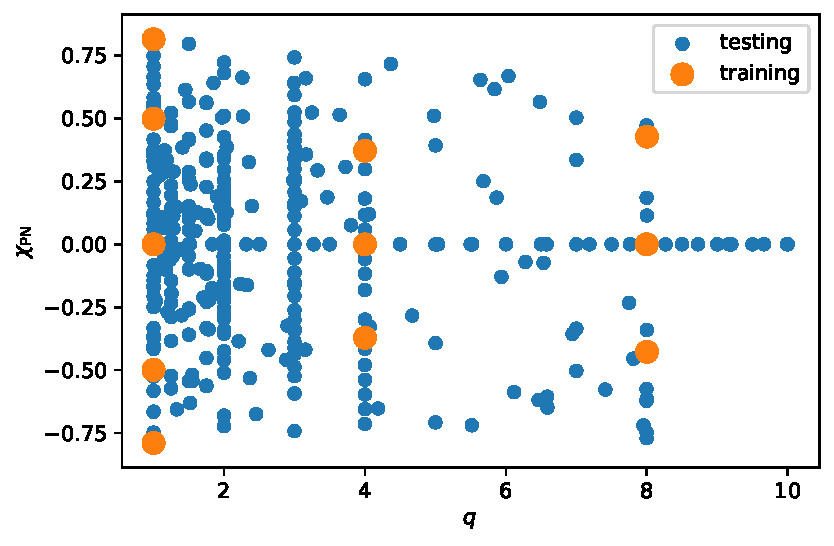
\includegraphics[width=\columnwidth]{figures/intrin_space.pdf}
	\caption{Distribution of training and testing waveforms in $q-\chi_{PN}$
	space. The blue dots represent the waveforms used in training and the orange
	stars represent the waveforms used in testing.\kw{Change the legend, and include the extra points. Change the training point to be star and testing point to be dot.}}
	\label{fig:intrin_space}
\end{figure}

\begin{table}[t]
	\centering
	\begin{tabularx}{0.8\columnwidth}{@{\extracolsep{\fill}}lrrr}
		\toprule\midrule Code         & $q$ & $\chi_1$ & $\chi_2$ \\
		\midrule\midrule SXS:BBH:0156 & 1.0 & -0.95    & -0.95    \\
		SXS:BBH:0151 & 1.0 & -0.60    & -0.60    \\
		SXS:BBH:0001 & 1.0 &  0.00    &  0.00    \\
		SXS:BBH:0152 & 1.0 &  0.60    &  0.60    \\
		SXS:BBH:0172 & 1.0 &  0.98    &  0.98    \\
		SXS:BBH:1418 & 4.0 & -0.40    & -0.50    \\
		SXS:BBH:0167 & 4.0 &  0.00    &  0.00    \\
		SXS:BBH:1417 & 4.0 &  0.40    &  0.50    \\
		SXS:BBH:0064 & 8.0 & -0.50    & -0.46    \\
		SXS:BBH:0063 & 8.0 &  0.00    &  0.00    \\
		SXS:BBH:0065 & 8.0 &  0.50    &  0.46    \\ \midrule\bottomrule
	\end{tabularx}
	\caption{List of waveforms used to recalibrate the model. The mass ratio
	$q=m_1/m_2\geq 1$ with spins $\chi_{1,2}$. Out of the 11 waveforms listed
	here, 9 of them are also used in the original IMRPhenomD calibration.
	\citep{khan2016frequency}}
	\label{tab:q148}
\end{table}
\begin{table}[t]
	\centering
	\begin{tabularx}{0.8\columnwidth}{@{\extracolsep{\fill}}lrrr}
		\toprule\midrule Code         & $q$ & $\chi_1$ & $\chi_2$ \\
		\midrule\midrule SXS:BBH:0234 & 2.0 & -0.85    & -0.85    \\
		SXS:BBH:0235 & 2.0 & -0.60    & -0.60    \\
		SXS:BBH:0169 & 2.0 & 0.00     & 0.00     \\
		SXS:BBH:0256 & 2.0 & 0.60     & 0.60     \\
		SXS:BBH:0257 & 2.0 & 0.85     & 0.85     \\ \midrule\bottomrule
	\end{tabularx}
	\caption{Additional waveforms used in further recalibration.}
	\label{tab:q1248}
\end{table}

\begin{figure*}[t]
	\script{0154.py}
	\centering
	\includegraphics[width=\textwidth]{figures/0154.pdf}
	\caption{Comparison between original and optimized IMRPhenomD waveforms.
	Here shows the SXS:BBH:0154 NR waveform, which has mass ratio $q=1$ and
	$\chi_1=\chi_2=-0.8$. The original mismatch is around $2.8\times10^{-4}$ and
	the optimized mismatch is around $5.3\times10^{-5}$. Top: It shows the
	amplitude and phase of NR, original IMRPhenomD and optimized IMRPhenomD
	waveform. Bottom: It shows the relative error of amplitudes between NR and
	IMRPhenomD waveforms, and the absolute error of phases between NR and
	IMRPhenomD waveforms}
	\label{fig:0154}
\end{figure*}

\section{Result and Comparison with Original Model} \label{sec:result}

To evaluate how well the optimization procedure generalize to waveforms that are
not in the training set, we evaluate the mismatch between the fine-tuned model
and the data provided in the SXS catalog for 536 NR waveforms. We select
waveforms that share the same part of the parameter space with the training
waveform, i.e. the waveforms with negligible eccentricity (${e<2\times10^{-3}}$)
and precession (${\chi_{x,y}<5\times10^{-3}}$). Fig.~\ref{fig:intrin_space}
shows how the training and testing waveforms are distributed in the
$q-\chi_{PN}$ space.

To illustrate the effect of optimiziation on an individual waveform level, we
compare the mismatch of a particular waveform before and after optimization with
respect to the NR waveform taken directly from the SXS catalog in Fig.
\ref{fig:0154}. Compared to the original IMRPhenomD waveform, the
optimized waveform has smaller residual from NR waveform both in amplitude and
phase, particularly in the inspiral region, where the amplitude displays a
$50\%$ reduction in error. For a fair comparison, we selected one of the testing
waveforms from the catalog presented in \citep{khan2016frequency}.

With the purpose of improving downstream tasks such as parameter estimation in
mind, the more relevant metric of improvement is the distribution of improvement
in mismatch over the entire training dataset. Fig. \ref{fig:q148} shows the
distribution of log-mismatch for the testing waveforms before and after the
optimization procedure. For generality, we use a constant PSD in our loss
function. One can see the distribution have been skewed toward lower mismatch,
where the peak of the distribution is shifted by approximately an order of
magnitude, and a median mismatch is reduced by 50\%. When using
$\mathcal{L}_{\mathrm{nl}}$, we observe a similar improvement with a 22.9\%
decrease in the median. 

\begin{figure}[t]
	\script{q148.py}
	\centering
	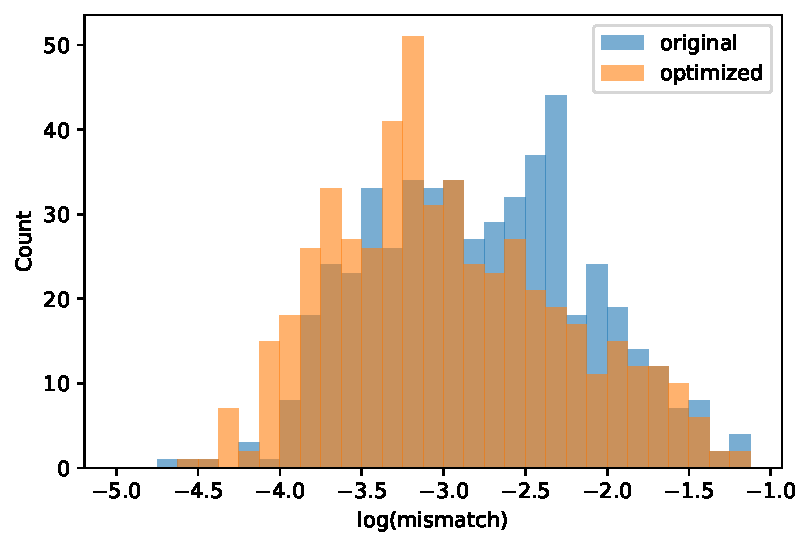
\includegraphics[width=\columnwidth]{figures/q148.pdf}
	\caption{Distributions of waveform mismatches calculated using 
	$\mathcal{L}_{\mathrm{ave}}$. We use training waveforms listed in 
	Tab.~\ref{tab:q148} and	mismatches are weighted with the constant PSD. 
	Dashed lines represent the median of the distributions, which has decreased by 45.3\%.}
	\label{fig:q148}
\end{figure}
\begin{figure}[t]
	\script{q148_q1248_compare.py}
	\centering
	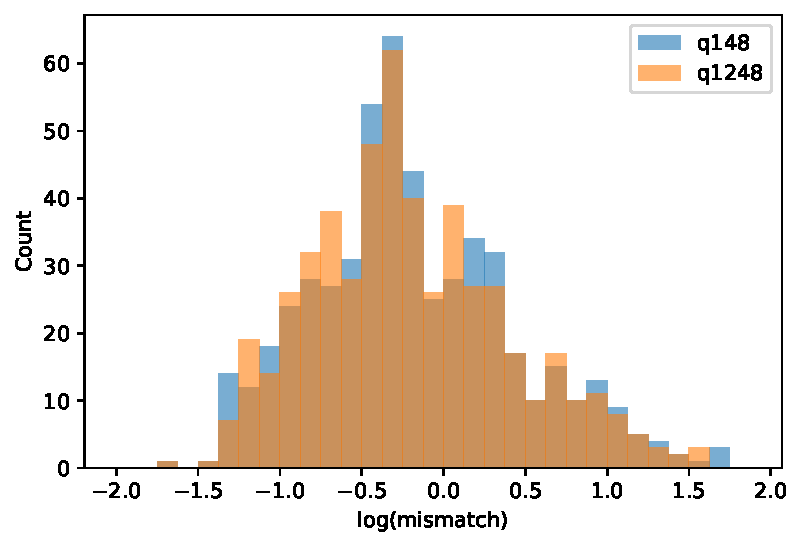
\includegraphics[width=\columnwidth]{figures/q148_q1248_compare.pdf}
	\caption{Distributions of $\log_{10}$ difference in mismatch. The
	distribution labeled \texttt{q148} uses training waveforms listed in
	Tab.~\ref{tab:q148} while the \texttt{q1248} distribution uses waveforms
	listed in Tab.~\ref{tab:q148}~and~\ref{tab:q1248}. Mismatches are calculated
	using the constant PSD with the loss function $\mathcal{L}_{\mathrm{ave}}$. 
	Dashed lines represent the median of the distributions, which has decreased by 10.4\%.}
	\label{fig:q148_q1248_compare}
\end{figure}

Note that the IMRPhenomD model was initially constructed and fitted using the
{\zdethp} weighted mismatch. To ensure a fair comparison, we apply the same
methods using the {\zdethp} PSD exhibit superior improvement compared to the
unweighted mismatch. We find no significant qualitative and quantitative
difference between the two PSDs in the resulting distribution of mismatches.

To understand whether additional training data can further improve the
performance of the model, we include waveforms that are not presence in the
original IMRPhenomD calibration in our training dataset with parameters
tabulated in Tab. \ref{tab:q1248}. We specifically choose to use $q=2$ events
since we have abundant $q=2$ NR waveforms to validate the final result. The new
set of coefficients generated from this optimization process yields only
marginal improvements in the newly produced waveforms, as seen in Fig.
\ref{fig:q148_q1248_compare}. The high mismatch tail of the optimized
distribution remains comparable to the original distribution, indicating that
the original dataset is sufficient for this task. Similarly, utilizing the
{\zdethp} PSD to optimize the loss function with additional waveforms results in 
similar level of improvement.

To investigate the performance of recalibration over the source parameter space,
we plot the improvement of mismatch in log projected over the parameter space of
$q$ vs. $\chi_{\mathrm{PN}}$ in Fig. \ref{fig:ps_q148_qchi}. On the mass ratio
axis, we can see the waveforms with $q\le4$ show most consistent average
improvement. This is because that part of the parameter space is better covered
by the training waveform, as compared to testing waveforms from $q=4$ to $q=8$,
where some testing waveforms lie outside the source parameter space covered by
the training set of waveforms. On the spin axis, we can see the waveform with
$\chi_{\textrm{PN}}$ close to zero show the most consistent improvement, and we
start deviate from 0, there could be fluctuations in the average improvement. On
top of that, in the $q\le4$ region, there seems to be more consistent
improvement of waveforms with $\chi_{\textrm{PN}}<0$. This can be understood as
since the original waveform was developed for aligned spin system, the waveforms
with $\chi_{\textrm{PN}}$ is less well-fitted \kw{Varify this.}, hence there
could be more room for improvement. To show this, we plot the parameter space of
$\chi_1$ vs. $\chi_2$ in Fig.~\ref{fig:ps_q148}. Waveforms along the diagonal
axis, i.e. $\chi_1\approx\chi_2$, show good mismatch improvements as discussed
above. Meanwhile, the top-left ($\chi_1<0<\chi_2$) and bottom-right
($\chi_1>0>\chi_2$) regions respond to optimization differently. In the top-left
region, waveforms generally improve slightly with along optimization. However,
waveforms in the bottom-right region do not improve after optimization. Some
waveforms even turned worse after optimization. 

 Given that the waveform model's ansatz may not be entirely compatible with NR,
and the optimization procedure is carried out over a distribution of waveforms
with varying source parameters, it is conceivable that different parts of the
source parameter space may not share the same set of optimal IMRPhenomD
parameters, mean there could be some trade-offs in accuracy between different
parts of the parameter space. If this is the cause of the lack of improvement in
the high mismatch tail of the distribution, segmenting the parameter space into
smaller subspaces should alleviate this problem. On the other hand, if the
ansatz lacks the correct parameterized form to capture the NR waveforms'
behavior as a function of the source parameters, the results will always be
biased, and we should not expect any improvement, even if we segment the
parameter space during training.


\begin{figure}[t]
	\script{ps_q148_qchi.py}
	\centering
	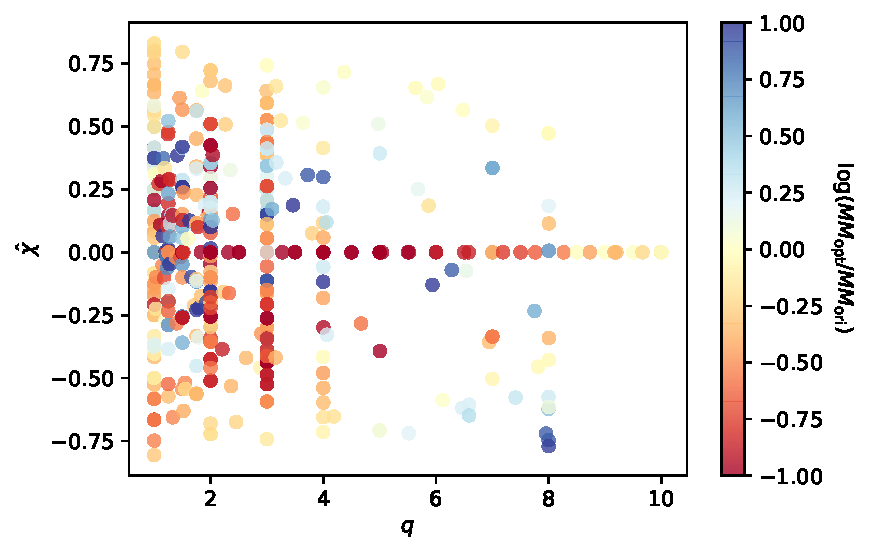
\includegraphics[width=\columnwidth]{figures/ps_q148_qchi.pdf}
	\caption{Parameter space of testing waveforms with $q$ against $\chi_{\mathrm{PN}}$. 
	We show the result from optimizing $\mathcal{L}_{\mathrm{ave}}$ with constant PSD 
	and training waveforms in Tab.~\ref{tab:q148}. Here, the colorbar represents the 
	$\log_{10}$ difference between optimized and original mismatches.}
	\label{fig:ps_q148_qchi}
\end{figure}
\begin{figure}[t]
	\script{ps_q148_chi1chi2.py}
	\centering
	\includegraphics[width=\columnwidth]{figures/ps_q148_chi1chi2.pdf}
	\caption{Parameter space of testing waveforms with $\chi_1$ against $\chi_2$. We
	show the result from optimizing $\mathcal{L}_{\mathrm{ave}}$ with the
	constant PSD and training waveforms listed in Tab.~\ref{tab:q148}.}
	\label{fig:ps_q148}
\end{figure}

\begin{table}[t]
	\centering
	\begin{tabularx}{0.8\columnwidth}{@{\extracolsep{\fill}}lrrr}
		\toprule\midrule Code         & $q$ & $\chi_1$ & $\chi_2$ \\
		\midrule\midrule SXS:BBH:0172 & 1.0 & 0.98     & 0.98     \\
		SXS:BBH:0152 & 1.0 & 0.60     & 0.60     \\
		SXS:BBH:0001 & 1.0 & 0.00     & 0.00     \\
		SXS:BBH:1417 & 4.0 & 0.40     & 0.50     \\
		SXS:BBH:0167 & 4.0 & 0.00     & 0.00     \\
		SXS:BBH:1426 & 8.0 & 0.48     & 0.75     \\
		SXS:BBH:0063 & 8.0 & 0.00     & 0.00     \\ \midrule 
		SXS:BBH:0370 & 1.0 & -0.20    & 0.40     \\
		SXS:BBH:2092 & 1.0 & -0.50    & 0.50     \\
		SXS:BBH:0330 & 1.0 & -0.80    & 0.80     \\
		SXS:BBH:2116 & 2.0 & -0.30    & 0.30     \\
		SXS:BBH:2111 & 2.0 & -0.60    & 0.60     \\
		SXS:BBH:0335 & 2.0 & -0.80    & 0.80     \\
		SXS:BBH:0263 & 3.0 & -0.60    & 0.60     \\
		SXS:BBH:2133 & 3.0 & -0.73    & 0.85     \\
		SXS:BBH:0263 & 4.0 & -0.80    & 0.80     \\ \midrule 
		SXS:BBH:0156 & 1.0 & -0.95    & -0.95    \\
		SXS:BBH:0151 & 1.0 & -0.60    & -0.60    \\
		SXS:BBH:0001 & 1.0 & 0.00     & 0.00     \\
		SXS:BBH:1418 & 4.0 & -0.40    & -0.50    \\
		SXS:BBH:0167 & 4.0 & 0.00     & 0.00     \\
		SXS:BBH:1419 & 8.0 & -0.80    & -0.80    \\
		SXS:BBH:0063 & 8.0 &  0.00    &  0.00    \\ \midrule 
		SXS:BBH:0304 & 1.0 & 0.50     & -0.50    \\
		SXS:BBH:0327 & 1.0 & 0.80     & -0.80    \\
		SXS:BBH:2123 & 2.0 & 0.30     & -0.30    \\
		SXS:BBH:2128 & 2.0 & 0.60     & -0.60    \\
		SXS:BBH:2132 & 2.0 & 0.87     & -0.85    \\
		SXS:BBH:2153 & 3.0 & 0.30     & -0.30    \\
		SXS:BBH:0045 & 3.0 & 0.50     & -0.50    \\
		SXS:BBH:0292 & 3.0 & 0.73     & -0.85    \\ \midrule\bottomrule
	\end{tabularx}
	\caption{List of waveforms used in recalibrating coefficients in 4 regions. From top to down are the top-right ($\chi_1,\chi_2>0$), top-left ($\chi_1<0<\chi_2$), bottom-left ($\chi_1,\chi_2<0$) and bottom-right ($\chi_1>0>\chi_2$) regions. Note that for the top-right and bottom-left regions, waveforms are chosen to have $\chi_1\approx\chi_2$, while the training waveforms for the other two regions are chosen to have $\chi_1\approx-\chi_2$.}
	\label{tab:quadrants}
\end{table}

We divided the parameter space into four regions to analyze the effect of the
recalibration procedure on each region separately
(Fig.~\ref{fig:ps_q148_quadrant}). The training waveforms used for fitting in
this scenario are listed in Tab.~\ref{tab:quadrants} and the loss functions 
are calculated using simple average of the mismatches. The top-left and
bottom-right regions have limited data for $q>4$, hence the results are only
valid up to $q\lesssim4$. From Fig.~\ref{fig:ps_q148_quadrant}, we observe that
equal-spin waveforms lying on the diagonal has great improvement. The
improvement above the diagonal is also substantial compared to recalibrate using
all waveforms at once, barring a few caused by some testing waveforms having
$q>4$. This can be seen clearer in Fig.~\ref{fig:all_quadrants}, which we see
that the optimized histogram shifts downward uniformly. On the other hand, the
improvement below the diagonal is negligible, indicating our method struggles to
further improve on top of the original IMRPhenomD waveform. Interestingly, we
can see in the top-right and bottom-left quadrant, the lower right corner shows
systematic worsening similar to the case of all waveforms. This hinted in
general, the IMRPhenomD waveform ansatz does not fit well with waveforms with
anti-aligned spin where the primary spin is positive.

\begin{figure}[t]
	\script{all_quadrants.py}
	\centering
	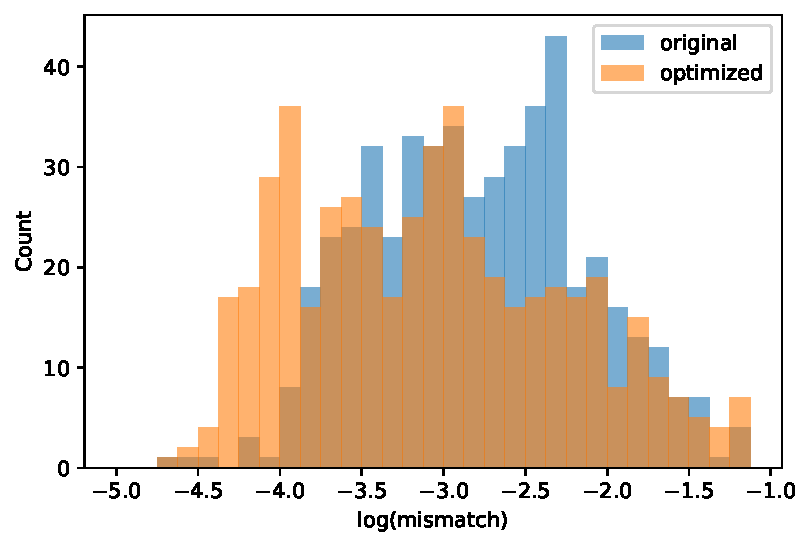
\includegraphics[width=\columnwidth]{figures/all_quadrants.pdf}
	\caption{Distributions of mismatches in the top-left (Top) and bottom-right
	(Bottom) regions. We use a constant noise spectrum to calculate mismatch and
	$\mathcal{L}_{\mathrm{ave}}$ as the loss function. Waveforms in the
	top-left region generally improves while waveforms in the bottom-right
	region has very little improvement, as indicated by the median (dashed
	lines). \kw{Is the original referring to original IMRPhenomD or optimized
	using everything? Can we have a reference for optimizing using everything?}}
	\label{fig:all_quadrants}
\end{figure}

\begin{figure}[t]
	\script{ps_q148_quadrants.py}
	\centering
	\includegraphics[width=\columnwidth]{figures/ps_q148_quadrants.pdf}
	\caption{Parameter space of testing waveforms. Each region is fitted independently with waveforms listed in Tab.~\ref{tab:quadrants}.}
	\label{fig:ps_q148_quadrant}
\end{figure}

\section{Discussion} \label{sec:discussion}

We have shown the result of recalibrating waveform coefficients. One thing to
note is that our recalibration procedure is not exactly the same as the original
calibration. For instance, we use a different set of NR waveforms, frequency
range, etc. Nonetheless, as the decrease in mismatch is rather significant, this
optimization procedure should be able to improve the accuracy of IMRPhenomD on a
similar scale regardless of the differences. Here, the result serves as a
demonstration of the general method used.  

The results presented in Fig.~\ref{fig:q148_q1248_compare} demonstrate that
increasing the number of training waveforms used in waveform optimization yields
only a marginal increase in accuracy. Our analysis suggests that this marginal
improvement is a consequence of over-determination of the waveform coefficients.
Consequently, increasing the number of calibration NR waveforms is unlikely to
result in any significant improvement of the model's accuracy. These
observations suggest that the parameterized ansatz employed in our study may not
be suitable for certain regions in the parameter space, leading to low mismatches
for some waveforms while other waveforms remain at the high mismatch tail with
negligible changes. This highlights the constraints of the model's flexibility
that ultimately limit its performance.

The reduced spin approximation is a major contributor to the inaccuracies
observed in the ansatz. In IMRPhenomD, this approximation employs a single spin
parameter, $\chi_{\mathrm{PN}}$, as described in Sec.~\ref{sec:method}. The
parameterization of BBH mergers using a single spin parameter results in a
degeneracy within the parameter space. Specifically, black hole events with
different spins may generate the same waveform due to identical values of
$\chi_{\mathrm{PN}}$, leading to erroneous results, particularly for highly
unequal spin events. This degeneracy produces straight lines in the parameter
space with negative slopes that depend on the mass ratio, which can be seen in 
Fig.~\ref{fig:ps_q148}. Notably, the ansatz performs better in the top-left
region than the bottom-right region. In an attempt to address
this issue, we partitioned the parameter space into four regions, as described
in Sec.~\ref{sec:result}. With separate optimizations for each
regions, Fig.~\ref{fig:ps_q148_quadrant} indicates that the top-left region's 
performance has improved, while the bottom-right region hardly improves. 
This observation suggests the ansatz is specific to certain regions of the 
parameter space, with a preference for BBH events lying above the diagonal, 
and it has limited enhancement for events lying below the diagonal. 

The division of the parameter space into four regions was a simple approach
taken for practical reasons. A more systematic approach would involve the use of
level set estimation algorithms to identify regions of interest within the
parameter space. Such an algorithm can reveal additional degeneracies or issues
that may exist within the ansatz. One possible strategy is to recalibrate
individual regions of interest to achieve better results. An alternative
approach is to select regions based on degeneracy lines. However, due to the
limited number of NR waveforms available, we were unable to implement this
approach. With more NR waveforms available in the future that cover the entire
parameter space, we can perform optimization with fewer restrictions and select
regions more systematically. Other than how to divide regions of interest, the 
choice of training waveforms also affects the final results greatly. Note that 
the choice of training waveforms listed in Tab.~\ref{tab:quadrants} were taken 
arbitrarily to test the effectiveness of separate fitting. Hence, if one takes 
a different set of training waveforms over the parameter space, the result might 
give additional features that can test and explain IMRPhenomD better. 

Although our study primarily focused on the IMRPhenomD model, this simple yet
versatile approach can be applied to other differentiable GW models, such as the
IMRPhenomP \citep{hannam2014simple, khan2019phenomenological} or IMRPhenomX \citep{pratten2020setting,pratten2021computationally} 
models within the same family. By jointly optimizing a new set of coefficients,
it is expected that both models can be enhanced since they share similar
construction principles to the IMRPhenomD model. For instance, they also use PN
approximants as part of the ansatz in the inspiral segment. It will be interesting 
to recalibratethe IMRPhenomXAS model \citep{pratten2020setting}. Because it is
parameterized by an additional anti-symmetric spin parameter, it is expected not
to exhibit the degeneracy previously described. With the currently developing 
{\jax} IMRPhenomXAS model in {\ripple}, A more detailed investigation
may provide valuable insights into the systematics of the Phenom models.
Furthermore, this approach is applicable to other GW model families, such as NR
surrogate models or EOB models introduced in Sec. \ref{sec:intro}. Such an approach could 
simplify NR waveform calibration procedures and lead to the improvement of 
existing models.

% Moved down from intro
% In particular, we find it is easier IMRPhenomD
% favors certain parts of the parameter space. This means IMRPhenomD introduces
% systematic bias to other GW analysis tasks. This showcases the flaws of the
% ansatz and allows us to have a deeper understanding of Phenom models.  

\section{Conclusion} \label{sec:conclusion}

In this paper, we have presented a systematic method to recalibrate GW models.
This method utilizes {\jax}'s automatic differentiation to apply
derivative-based optimization to recalibrate GW models jointly. Using the new
implementation of the IMRPhenomD model, {\ripple}, which is written in \jax, in
conjunction with NR waveforms from the SXS catalog, we recalibrate waveform
coefficients of the IMRPhenomD model. In general, the waveform accuracy can be
improved by 50\%. Comparing {\zdethp} weighted and unweighted mismatch, weighted
mismatches have a slightly better improvement. In contrast, different types of
loss function result in significantly different final mismatch distributions. As 
seen in Fig.~\ref{fig:q148}, $\mathcal{L}_{\mathrm{ave}}$ outperforms 
$\mathcal{L}_{\mathrm{nl}}$. By increasing the number of training waveforms, we see a 
slight improvement increase in Fig.~\ref{fig:q148_q1248_compare}. 

Furthermore, we investigated how the source parameters affect the
improvement. Fig.~\ref{fig:ps_q148} shows that the optimization procedure has a
certain preference for waveforms lying in the top-left region while the bottom-right 
region hardly improved. To further test this result, we recalibrate
waveforms in separate regions in parameter space. From Fig.~\ref{fig:ps_q148_quadrant}, 
we can see that this recalibration process gives further
improvement to the top-left region while the bottom-right region only have little 
improvement. This indicates that the ansatz has limited match in this region and 
does not fit most waveforms in this region, hence introduces bias to downstream GW 
analysis. This phenomenon is mainly due to the reduced spin approximation used in 
parameterizing the ansatz, where degeneracies between $\chi_1$ and $\chi_2$ are introduced. 

While we naively separate the optimization process into 4 regions, one can
perform systematic region-selection. In principle, we can apply this general
method to other newer and more accurate models such as IMRPhenomX or IMRPhenomP
models. Then, we can perform all the above analyses to understand how to
construct better GW Phenom models in the future.  

\section{ACKNOWLEDGMENTS}

We thank Will M.~Farr, Max Isi, and Mark Hannam for helpful discussions; we also
thank Carl-Johan Haster, Neil J.~Cornish and Thomas Dent for comments on the
draft. The Flatiron Institute is a division of the Simons Foundation. T.E.\ is
supported by the Horizon Postdoctoral Fellowship.
\bibliography{bib}

\end{document}
